\label{chap:literature_review}

\section{Keywords and Thresholds}
\begin{center}
\begin{table}

  \begin{tabular}{c|c|c}
    \hline 
    Concept & Keywords & Articles Threshold\tabularnewline
    \hline 
    tabagism & lung nodule tabagism OR lung cancer tabagism & First 8\tabularnewline
    guidelines & lung screening guideline OR lung cancer guideline & First 8\tabularnewline
    lung cancer & lung cancer OR malignant lung nodule & First 8\tabularnewline
    \hline 
  \end{tabular}
\par
\caption{\label{table:search_terms} Search terms}
\end{table}
  \vspace*{-44pt}
\end{center}

The table \ref{table:search_terms} show all the search terms utilized as a basis to extract key articles from Google Scholar, Springer  and ScienceDirect resources. For each of these articles, the most interesting related documents were also taken into account.

For each of these articles, guidelines, books and documents evaluated only the first eight of each combined search was kept as a result. All were read and the most impacting related works were also taken into consideration for this systematic literature review.

So for only the three different combined search parameters, 24 papers were selected. From these each, the  most impacting cited ones were taken into consideration, increasing the number of papers to  read to 58. From this overall number, 10 were selected to be cited as part of the literature review. % TODO

\section{Lung Cancer Studies}

Lung Cancer is the type of 30\% of all cancers. From these 30\%, 90\% of these cancers are  caused by the fact that the patient is an active or recent smoker \cite{jaklitsch2012}\cite{nccn2019}\cite{roberts2013}. This is an important literature finding because it means that patients that are effective smokers will have much greater chance of developing lung cancer than other patients.

Not only that, but other studies found out that the average quit ratio on the entire smoker worldwide population is of 7\% only but when lung  cancer screening is taken into consideration, about 25\% of the patients that start in screening program are likely to quit smoking \cite{fox2003}\cite{aalst2010}. %TODO - smoking cessation paper too

\section{Imaging Lung Nodules}

Some of the papers mention the existence of a strong correlation between patient survivability for the first 24 months and the cancer development stage. It is so common to use cancer stage (I to IV) as a proxy for survivability that there are even works whose main focus is to uncover these relations\cite{roberts2013}\cite{fox2003}.

The extensive usage of low-dose computed tomography (LDCCT) scans are also the reason for up a 20\% increase in patient survivability for the first two years of the disease development\cite{fox2003}\cite{macredmond2006}\cite{mountain2008}\cite{jaklitsch2012}. The efficiency of such early stages screening programms for LDCCT was first shown by \citeonline{henschke1999} as part of the Early Lung Cancer Action  Project (ELCAP). In this project, Chest X-ray (CXR) had an overall efficiency of 68\% and LDCCT had a 95\% for non-calcified nodules. Malignant nodules were found in 27\% of LDCCT and only 7\% for CXR. 

Other works have not only focused on the efficiency and the role of imaging but also ono the patient risk profile which is strictly related to smoking behavior.

\section{The Role of Tabagism}

Tabagism stands as the root cause for 90\% of all lung cancers. There is an increased patient risk of developing lung cancer even for patients that smoke \cite{ostroff2001}\cite{aalst2010}\cite{aalst2011}. There is definitely incidence among never smokers too but it occurs with a much lesser frequency and develops slower, mostly if the patient quits smoking before or during the radiotherapy treatment \cite{fox2003}\cite{rivera2016}

Data on tabagism is often reported for some of the patients that happen to come for Chest X-ray and Chest CT (CCT). These patients will with frequency fill up forms that amongst other informations will also extract if the patient is a smoker or not, what he or she smokes and the quantity per year. This is also true for \nomeHsl{}. 

\section{Extracting Information from Reports}

Not all patient information is stored in the form of a structured form or in a restricted text field. That means that to extract valuable information insights from the radiology reports, the anatomy patalogy reports and so on it is necessary to make extensive use of Natural Language Processing (NLP). %TODO citations

It is a known  fact that most of the medical data, altough in digital format since decades, is still in free text fields. %TODO citations
So, additional data processing is indeed necessary to provide the basis for the extraction of actionable data from the reports.

\citeonline{fleischner2017} have defined the Fleischner 2017 radiology guideline that aims to provide a patient follow-up scenario in the case of an incidental nodule finding for it. \nomeHsl{} uses Fleischner extensively for all CCT and CXR. These two procedures constitute one of the most basic imaging procedures and they do correspond to almost 20\% of all imaging done at \nomeHslShort{}. %TODO

The Fleischner guideline defines different criteria depending on the lung nodule findings in the radiology reports. These criteria are displayed at tables \ref{tab:solid_nodules} and \ref{tab:subsolid_nodules} in detail. Each of the radiology findings could potentially have a follow-up that could or not occur in time.

\begin{center}
\begin{table}
\begin{centering}
\begin{tabular}{c|>{\centering}p{0.25\textwidth}|>{\centering}p{0.25\textwidth}|>{\centering}p{0.25\textwidth}}
\hline 
\multicolumn{4}{c}{Single}\tabularnewline
\hline 
Risk & $<6mm$ & $6-8mm$ & $>8mm$\tabularnewline
\hline 
Low Risk & No routine follow-up & CT at 6-12 months, then consider CT at 18-24 months & Consider CT at 3 months, PET/CT or tissue sampling\tabularnewline
High Risk & Optional CT at 12 months & CT at 6-12 months, then consider CT at 18-24 months & Consider CT at 3 months, PET/CT or tissue sampling\tabularnewline
\hline 
\multicolumn{4}{c}{Multiple}\tabularnewline
\hline 
Low Risk & No routine follow-up & CT at 6-12 months, then consider CT at 18-24 months & CT at 6-12 months, then consider CT at 18-24 months\tabularnewline
High Risk & Optional CT at 12 months & CT at 6-12 months, then consider CT at 18-24 months & CT at 6-12 months, then consider CT at 18-24 months\tabularnewline
\hline 
\end{tabular}
\par\end{centering}
\caption{\label{tab:solid_nodules} \emph{Solid nodules} follow-up table according to \citeonline{fleischner2017}.}
\end{table}
\vspace*{-44pt}
\par\end{center}

\begin{center}
\begin{table}
\begin{centering}
\begin{tabular}{c|>{\centering}p{0.35\textwidth}|>{\centering}p{0.35\textwidth}}
\hline 
\multicolumn{3}{c}{Single}\tabularnewline
\hline 
Risk & $<6mm$ & $\geq6mm$\tabularnewline
\hline 
Ground Glass & No routine follow-up & Consider CT at 3 CT at 6-12 months to confirm persistence, then CT
every 2 years until 5 years\tabularnewline
Part Solid & No routine follow-up & Consider CT at 3 months, PET/CT or tissue sampling\tabularnewline
\hline 
\multicolumn{3}{c}{Multiple}\tabularnewline
\hline 
High Risk & CT at 3-6 months, if stable consider CT at 2 and years & CT at 3-6 months. Subsequent management based on most suspicious node(s)\tabularnewline
\hline 
\end{tabular}
\par\end{centering}
\caption{\label{tab:subsolid_nodules}\emph{Subsolid nodules} follow-up table according
to \citeonline{fleischner2017}.}
\end{table}
\vspace*{-44pt}
\par\end{center}

\begin{center}
\begin{figure}
\begin{centering}
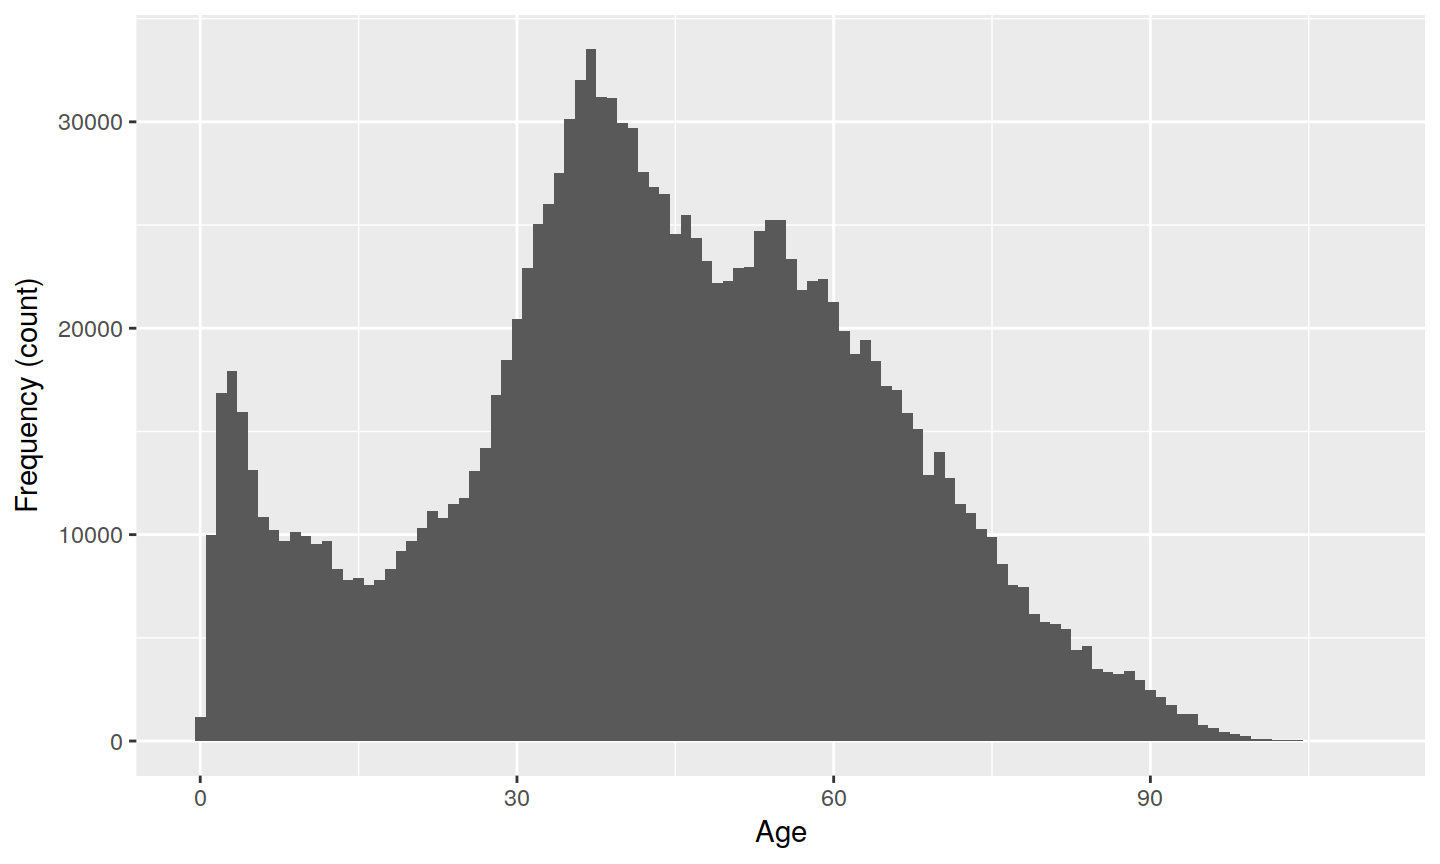
\includegraphics[width=0.5\textwidth]{PatientPopulation}
\par\end{centering}
\begin{centering}
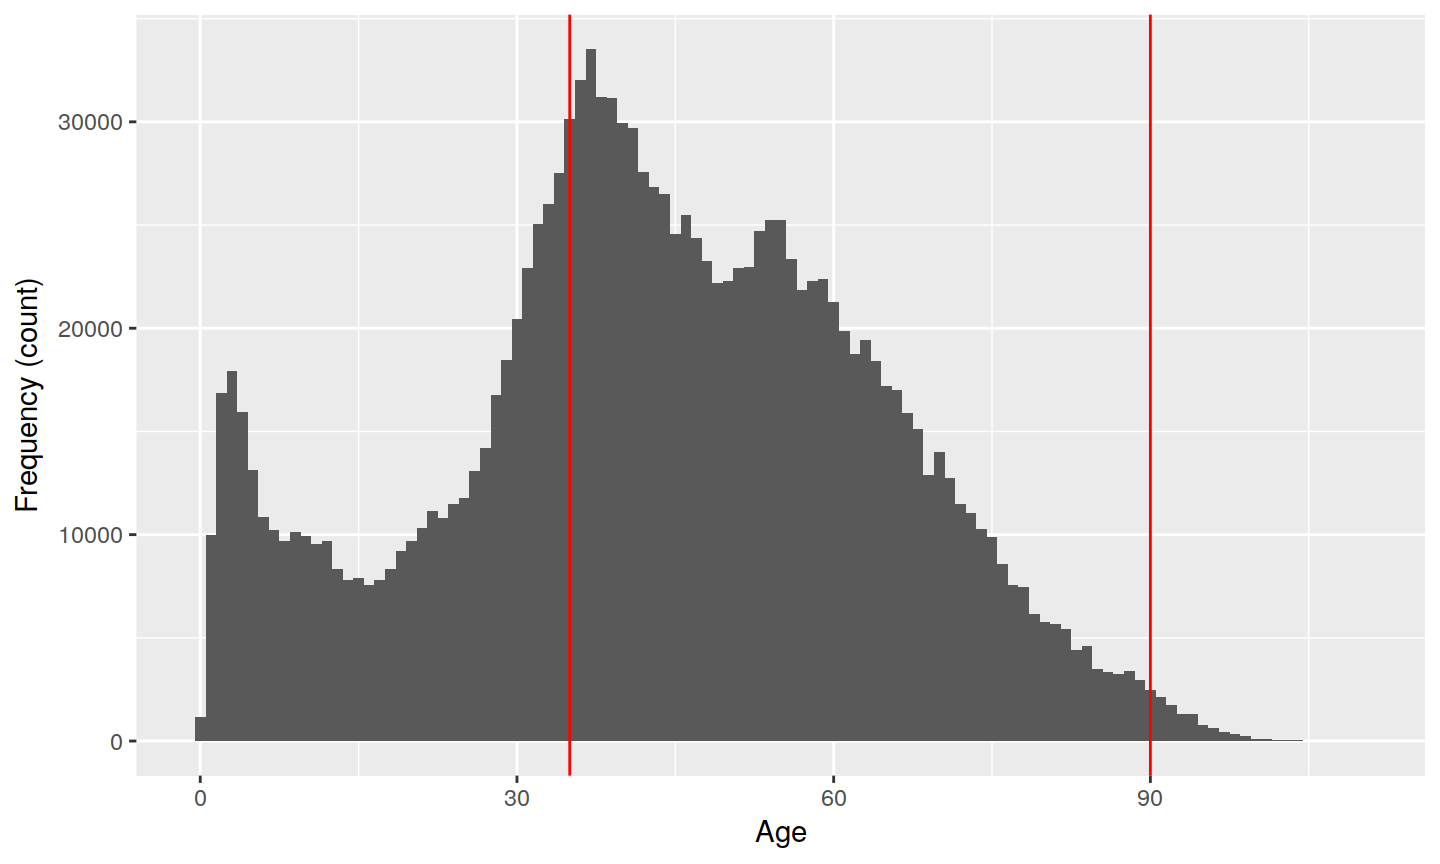
\includegraphics[width=0.49\textwidth]{PatientPopulationWithThreshold}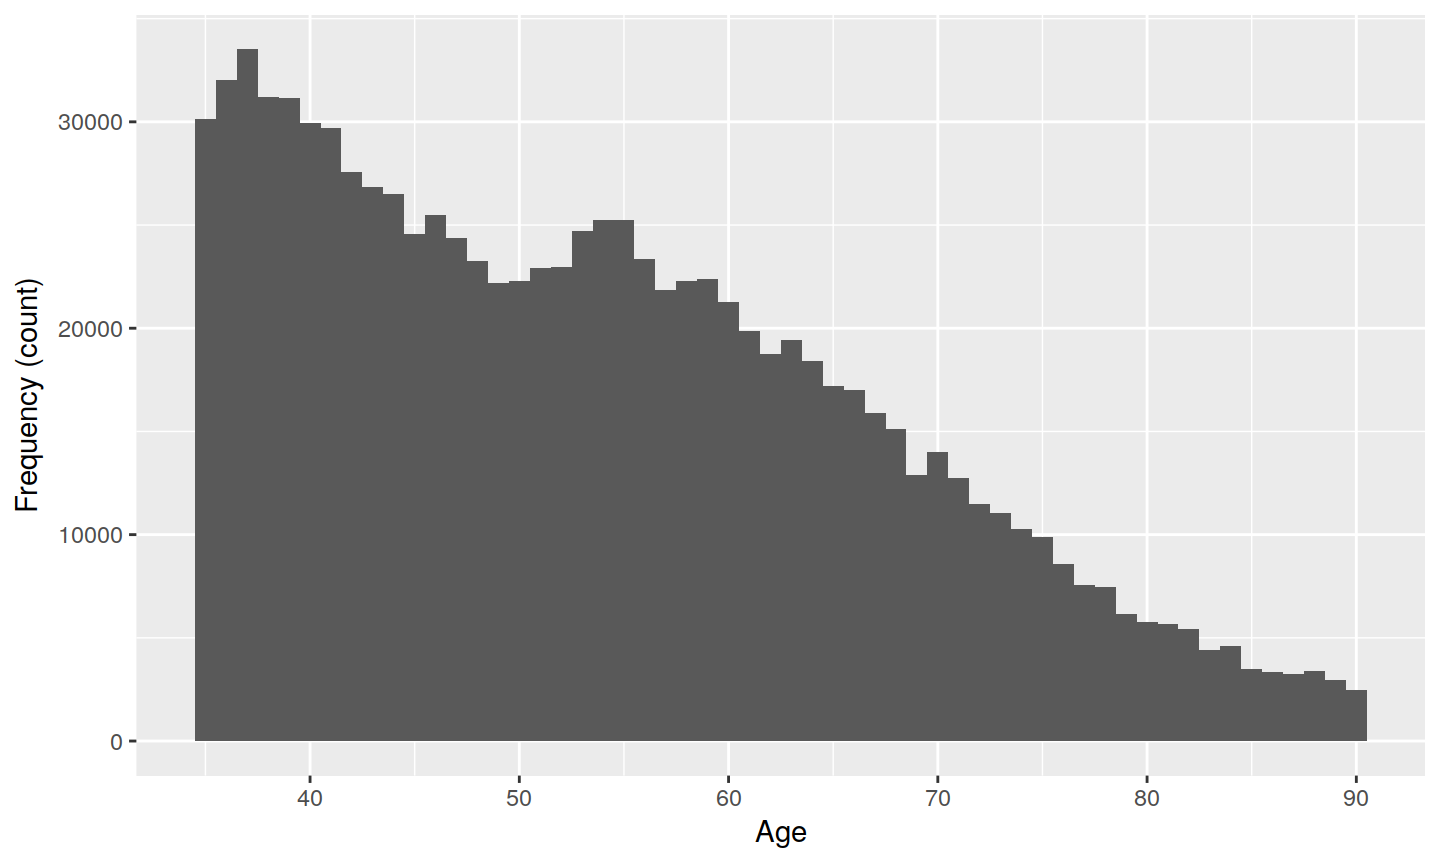
\includegraphics[width=0.49\textwidth]{FilteredLungNodulePopulation}
\par\end{centering}
\caption{\label{fig:patient_population}The upper histogram defines the whole \nomeHsl{} population. The lower left image shows a vertical bar on 35 and 90 years which can
be considered minimum and maximum bounds for patient screening and
finally the lower right image is a filtered version of the lower left
histogram only taking the age intereval of interest into consideration.}
\end{figure}
\vspace*{-44pt}
\par\end{center}

These follow-ups should occur as a  means of mitigating the risk that the risk of finding a malignant cancer in a late stage of clinical evolution. Missed follow-ups, as mentioned in  the chapter \ref{chap:introduction} are one of the possible medical errors. These are especially common when taking radiology reports into consideration. The reason for it is that the ordering or referring physician for the image exam forgets or does not reads the incidental lung nodule finding. 

So it would be appropriate to have any tool to help both the ordering or referring physician and the responsible physician at \nomeHsl{}. This holds true as about one third of \nomeHslShort{} workforce is constituted of external physicians, decreasing precision medicine returns values for itself. For that matter, the use of the information stored at \nomeHslShort{} has the potential of solving a potential care gap. 

\section{Differentiating Risks}

As mentioned in the previous sections, the existence of both a radiology report based risk profile and the follow-up table depending basically on the lung nodule type and  size (tables \ref{tab:solid_nodules} and \ref{tab:subsolid_nodules}). 

The patient family history of cancer and also it's smoking behavior and age should provide insight on wether the patient should be screened or not and that is the endgoal of this work.

The figure \ref{fig:patient_population} shows the overall patient population for the institution. The suggested patient population filters are based on \nomeHslShort{} own internal guidelines along with the Fleischner 2017 and NCCN recommendations.

Also, a 10 pack-year smoking history qualifies the patient for a routine follow up after 35 years as mentioned for \nomeHslShort{}. In that sense, the figure \ref{fig:cigars_per_day} an overall picture of the patient smoking behavior for the hospital's own population is given. In this dataset, only 24\% of all screeneable patients can be considered smokers which is only slightly lower than the wolrdwide average of 30\% smokers.

\begin{center}
\begin{figure}
\begin{centering}
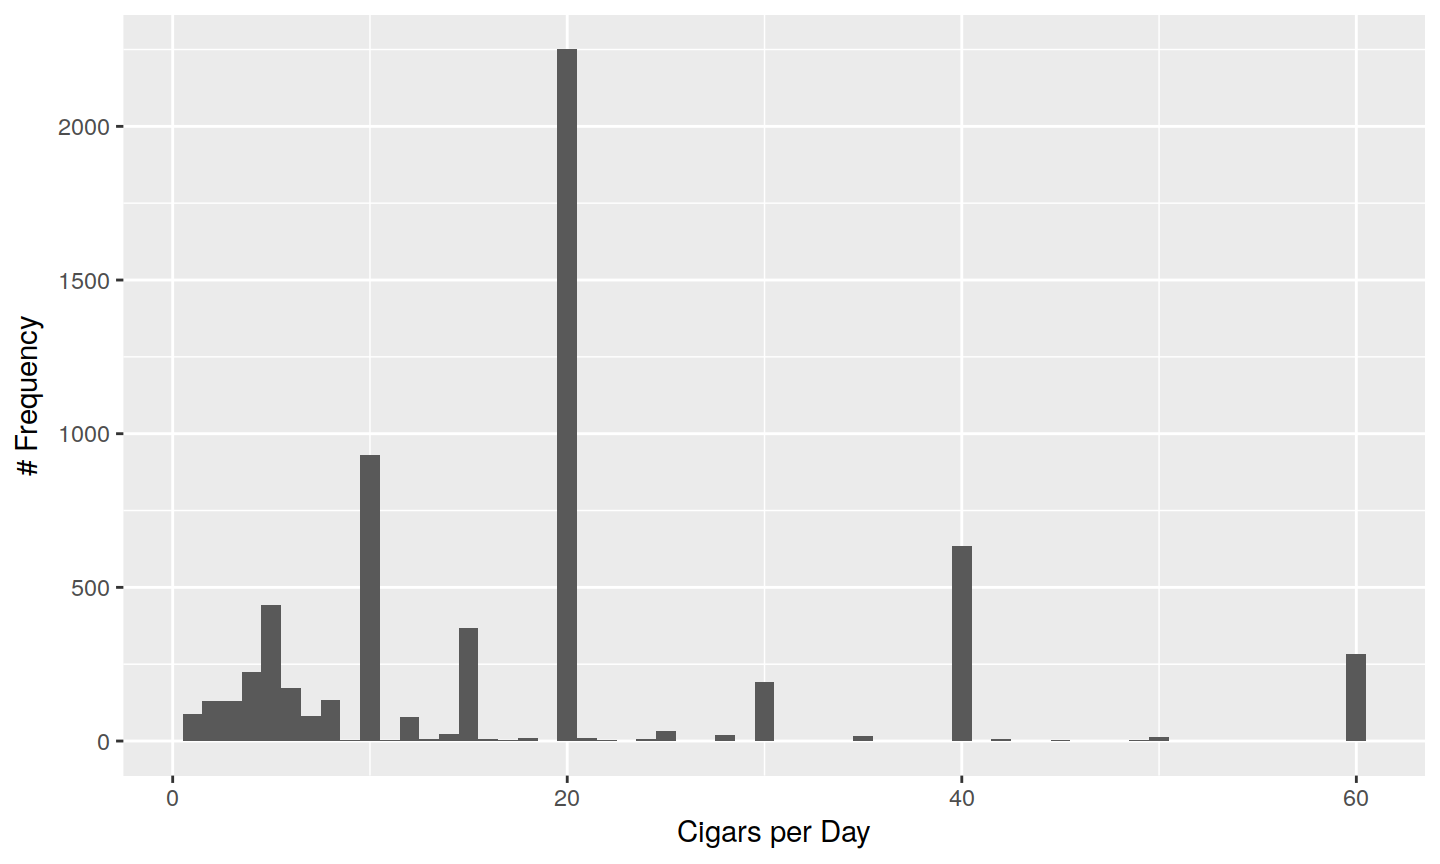
\includegraphics[width=1\textwidth]{PatientsCigarsPerDay}
\par\end{centering}
\caption{\label{fig:cigars_per_day} Histogram of cigars per day according to \nomeHsl{} own internal's
patient autoreported information.}
\end{figure}
\vspace*{-44pt}
\par\end{center}

